\documentclass[12pt]{article}
\title{Inferring generation-interval distributions from contact tracing data: \\ \emph{in prep, PRSB}}
\author{Sang Woo Park, David Champredon and Jonathan Dushoff}

\usepackage{graphics}
\usepackage{adjustbox}

\newcommand{\eref}[1]{(\ref{eq:#1})}
\newcommand{\fref}[1]{Fig.~\ref{fig:#1}}
\newcommand{\Fref}[1]{Fig.~\ref{fig:#1}}
\newcommand{\sref}[1]{Sec.~\ref{#1}}
\newcommand{\frange}[2]{Fig.~\ref{fig:#1}--\ref{fig:#2}}
\newcommand{\tref}[1]{Table~\ref{tab:#1}}
\newcommand{\tlab}[1]{\label{tab:#1}}

\usepackage{amsthm}
\usepackage{amsmath}
\usepackage{amssymb}
\usepackage{amsfonts}

\usepackage{hyperref}
\usepackage{natbib}
\usepackage{hyperref}
\bibliographystyle{chicago}
\date{\today}

\usepackage{xspace}
\newcommand*{\ie}{i.e.\@\xspace}

\usepackage{color}

\newcommand{\Rx}[1]{\ensuremath{{\mathcal R}_{#1}}} 
\newcommand{\Ro}{\Rx{0}}
\newcommand{\RR}{\ensuremath{{\mathcal R}}}
\newcommand{\tsub}[2]{#1_{{\textrm{\tiny #2}}}}

\newcommand{\comment}[3]{\textcolor{#1}{\textbf{[#2: }\textsl{#3}\textbf{]}}}
\newcommand{\jd}[1]{\comment{cyan}{JD}{#1}}
\newcommand{\swp}[1]{\comment{magenta}{SWP}{#1}}
\newcommand{\dc}[1]{\comment{blue}{DC}{#1}}
\newcommand{\hotcomment}[1]{\comment{red}{HOT}{#1}}

\begin{document}
\maketitle

\section{Introduction}

An epidemic can be characterized by its speed (exponential growth rate, $r$) and its strength (reproductive number, \RR).
Reproductive number, defined as the average number of secondary cases arising from a primary case, is of particular interest as it provides information about the final size of an epidemic [CITE].
However, directly measuring the reproductive number often requires detailed knowledge of disease natural history and may not be feasible early in an epidemic [CITE].
Instead, the reproductive number can be \emph{indirectly} estimated from exponential growth rate, which can easily be estimated from incidence data [CITE].
These two quantities are linked by generation-interval distributions \citep{wallinga2007generation}.

Generation interval is defined as the time between when a person becomes infected and when that person infects another person.
Due to individual variation in infection time, the observed generation-interval distribution can change depending on when and how it is measured \citep{svensson2007note, kenah2008generation, nishiura2010time}.
There are important distinctions to be made when estimating generation intervals: \emph{intrinsic} generation intervals are measured by evaluating the infectiousness of infected people,
%% without regard to actual infection events,
while \emph{observed} generation intervals refer to the time between actual infection events.
Observed generation intervals in turn can be \emph{aggregated} across time, measured \emph{forward} in time by looking at a cohort of individuals infected at the same time and asking when they infected others, or measured \emph{backward in time} by look at a cohort and asking when their infectors were infected \citep{champredon2015intrinsic}.
% When aggregated generation intervals are observed until a given time in an ongoing epidemic (often via contact tracing), we refer to these as \emph{censored} (or right-censored) intervals.

Early in the epidemic when depletion of susceptible is negligible, we expect the forward generation-interval distribution to be similar to the intrinsic generation-interval distribution.
As epidemic progresses, an infector is less likely to infect individuals later in time due to decrease in susceptibles and the distribution of forward generation intervals will be shorter than the intrinsic distribution.
Conversely, when an epidemic is growing exponentially, as often occurs near the beginning of an outbreak, the number of newly infected individuals will be large relative to the number infected earlier on. 
A susceptible individual is thus relatively more likely to be infected by a newly infected individual, and the distribution of backward generation intervals will be shorter than the intrinsic distribution.
When epidemic is subsiding, most infections are caused by the remaining infectors, rather than new infectors, and the backward generation interval will be long.
\swp{Where can I cite champredon? First sentence? Last sentence? Or don't cite DC because I already did in the previous paragraph?}

In practice, generation intervals are measured by contact tracing throughout the course of an epidemic, usually aggregated to increase the amount of information available; we refer to these as \emph{censored} (or right-censored) intervals.
When calculations are based on early-outbreak data, the available (censored) observations can be thought of as a weighted average of backward generation-interval distributions; like them, the observed censored intervals will be shorter than intrinsic distributions.

Observed generation intervals also vary across space.
In a structured population (that is, any population that does not mix homogeneously), susceptibility will tend to decrease more quickly in  the neighborhood of infected individuals than in the general population. 
This means that contacts made late in infection are more likely to be ``masked'' due to contacts already being infected.
Therefore, realized generation intervals will be shorter and observed generation intervals may underestimate the intrinsic generation-interval distribution even when population-level susceptibility is very high.

This perspective allows us to reinterpret the finding of \cite{trapman2016inferring} that, given an intrinsic generation interval and an observed growth rate $r$, the reproductive number $\RR$ on various network structures is always smaller on a network than would be predicted from homogeneous mixing.
\jd{Maybe moving on a good direction, but needs more work. The problem is that we need to talk clearly about the spatial correction without misleading people about the temporal correction.}

\swp{Will rewrite this paragraph after writing the rest of it:}
In this study, we explore the temporal and spatial variation in the observed generation-interval distributions obtained from contact tracing.
We show that using the observed generation-interval distribution directly will always underestimate the reproductive number \swp{need to confirm this statement when we're done with the ms}. 
We provide a statistical framework of recovering the intrinsic generation-interval distribution from the observed generation-interval distribution.

\swp{Going to rename the sections... but I think I like the current order...}
\section{Generation-interval distributions across time}

\subsection{Intrinsic kernel}

We begin by introducing an analytical framework.
Let $K_a(\tau)$ be an individual-level intrinsic kernel, i.e., the rate at which secondary infections are expected to be caused by an individual $a$ \citep{svensson2015influence}; \swp{Need to say something more about Sven; come back later}
an individual-level intrinsic kernel describes an intrinsic infectiousness of an infected individual.
The population-level intrinsic kernel is given by integrating over individual variations:
\begin{equation}
K(\tau) = \int K_a (\tau) dA.
\end{equation}
The basic reproductive number -- average number of secondary cases caused by an average primary case in a fully susceptible population -- is defined as: 
\begin{equation}
\RR_0 = \int K(t).
\end{equation}
The intrinsic generation-interval is simply the population-level kernel normalized by the basic reproductive number:
\begin{equation}
g(\tau) = \frac{K(t)}{\RR_0}.
\end{equation}
Then, the renewal equation model can be used to model incidence over time:
\begin{equation}
i(\tau) = S(\tau) \int K(s) i(\tau-s) ds = \RR \int g(s) i(\tau-s) ds
\end{equation}
where $i(\tau)$ is incidence at time $\tau$ and $S(\tau)$ is the proportion of the population susceptible.
Finally, assuming exponentially growing incidence ($i(t) = i(0) \exp(r t)$), we obtain the Euler-Lotka equation [CITE]:
\begin{equation}
\frac{1}{\RR} = \int g(\tau) \exp(-r \tau) d\tau.
\end{equation}

\subsection{Right-censored intervals}

\jd{Have to set this up to make sure we're not sounding too mathy.}
Assume that contact tracing is performed from the beginning of an epidemic to time $t$.
The number of infection occuring at time $s$ caused by infectors who were themselves infected at time $s-\tau$ is given by
\begin{equation}
i_{s-\tau}(s) = \RR i(s-\tau) g(\tau) S(s)
\end{equation}
Then, total number of secondary infections that are $\tau$ time steps apart and occur before time $t$:
\begin{equation}
\RR \int_\tau^t i(s-\tau) g(\tau) S(s) ds.
\end{equation}
Then, the censored interval at time $t$ is given by
\begin{equation}
c_t(\tau)= \frac{\RR \int_\tau^t i(s-\tau) g(\tau) S(s) ds}{\RR \int_0^t \int_x^t i(s-x) g(x) S(s) ds dx}.
\end{equation}
We note that the expression in the denominater is equivalent to cumulative incidence at time $t$.
The intuition behind this is that we are normalizing acrosss all incidence before time $t$.
Then, we have
\begin{equation}
c_t(\tau) = \frac{\RR \int_\tau^t i(s-\tau) g(\tau) S(s) ds}{\int_0^t i(s) ds}.
\end{equation}
For convenience, we ignore normalizing constants and write
\begin{equation}\label{eq:obsg}
c_t(\tau) \propto g(\tau) \int_{0}^t i(s-\tau) S(s) ds.
\end{equation}

For a single epidemic, the observed mean generation interval through contact tracing will always be shorter than intrinsic mean generation interval (Figure~\ref{fig:censor}).
There are two reasons for this phenomenon.
First, any infection events that occur after the contact tracing period canonot be observed due to right censoring and short generation intervals are more likely to be observed.
In particular, when an epidemic is growing exponentially ($i(t) \propto \exp(rt)$), 
the censored generation-interval distribution is equivalent to the inverse exponentially weighted intrinsic generation-interval distribution:
\begin{equation}
\tsub{c}{exp}(\tau) \propto g(\tau) \exp(-r\tau).
\label{eq:exp}
\end{equation}
% As backward generation-interval distributions are always shorter than the intrinsic generation-interval distribution during the exponential growth period, their weighted average (i.e., the censored intervals) will also be shorter.
Second, decreasing number of susceptibles over the course of an epidemic makes long infections less likely to occur, and the realized intervals will always be shorter \citep{champredon2015intrinsic}.
As a result, even if contact tracing is performed through an entire epidemic, mean generation interval will be underestimated.

\begin{figure}
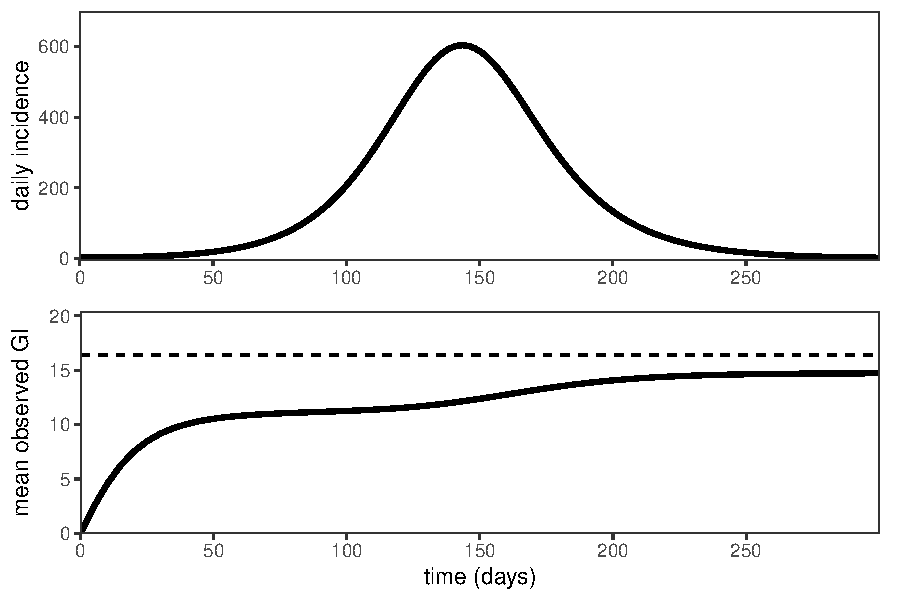
\includegraphics[width=\textwidth]{../fig/temporal_effect.pdf}
\caption{\textbf{Temporal variation in the mean observed generation interval.}
A deterministic Susceptible-Exposed-Infectious-Recovered (SEIR) model was simulated using Ebola-like parameters and the observed mean generation interval was calculated the course of an epidemic (see methods).
}
\label{fig:censor}
\end{figure}

When a disease is at (or near) endemic equilibrium, the number of susceptibles remains (approximately) constant over time, and the observed generation-interval distribution should be similar to the intrinsic generation-interval distribution.
\swp{Probably don't need a figure for this}

\section{Generation-interval distributions across space}

\subsection{Egocentric kernel}

Within a limited contact structure, a susceptible individual can be contacted multiple times;
infectious contacts give rise to infection only when the susceptible individual is contacted for the first time.
In particular, we can look at it from an egocentric point of view -- i.e., from a perspective of a single infector.
Then, we can define the egocentric kernel, i.e., the rate at which secondary infections are realized by a single primary case $a$:
\begin{equation}
\hat{K}_a(\tau) = K_a(\tau) \exp \left(- \delta_a \int_0^\tau K_a(s) ds\right),
\end{equation}
where $K_a(\tau)$ is the individual-level intrinsic kernel and $e^{- \delta_a \int_0^\tau K_a(s) ds}$ is the probability that a susceptible acquaintance has not yet been contacted by individual $a$.
The dilution term, $\delta_a$, models how contacts are distributed among susceptible acquaintances.
For example, when infectious contacts are distributed equally in a homogeneous population, we have $\delta_a = 1/(N-1)$, where $N$ is the population size.

The population-level egocentric kernel is given by integrating over individual variations:
\begin{equation}
\hat{K}(\tau) = \int \hat{K}_a(\tau) dA,
\end{equation}
and the population-level egocentric generation-interval distribution is:
\begin{equation}
\hat{g}(\tau) = \frac{\hat{K}(\tau)}{\int \hat{K} \tau}.
\label{eq:conditional}
\end{equation}
The population-level egocentric generation-interval distribution describes the distribution of times at which secondary infections are realized by an average primary case.
For convenience, egocentric distribution refers to the population-level distribution, unless noted otherwise.

For example, consider a susceptible-exposed-infected-recovered (SEIR) model.
This model assumes that latent and infectious periods are exponentially distributed and can describe wide range of diseases.
It has been shown that the intrinsic generation-interval distribution that corresponds to this model is given by [CITE]:
\begin{equation}
g(\tau) = \frac{\sigma \gamma}{\sigma - \gamma} \left(e^{-\gamma t} - e^{-\sigma t}\right),
\end{equation}
where $1/\sigma$ and $1/\gamma$ are mean latent and infectious periods, respectively.
Assuming that per-pair contact rate is $\lambda$ for any pair, we obtain the following egocentric generation-interval distribution is given by:
\begin{equation}
\hat{g}(\tau) = \frac{\sigma (\gamma + \lambda)}{\sigma - (\gamma + \lambda)} \left(e^{-(\gamma + \lambda)t} - e^{-\sigma t}\right)
\end{equation}
In this scenario, per-pair contact rate is effectively decreasing mean infectious period: an infected individual is can no longer infect anyone (hence no longer infectious) when all its susceptible acquaintances have ben infected.

The difference between egocentric and intrinsic generation-interval distribution can be demonstrated by simulating stochastic infection processes on a small tree network (i.e, a single infected individual is connected to multiple susceptible individuals who are not connected with each other) with artificially high per-pair contact rate.
Simulations confirm that in this case the distribution of contact times matches the intrinsic generation-interval distribution, while the distribution of realized generation times matches with the egocentric generation-interval distribution (\fref{fig:local}) -- generation times are shorter on average because contacts with already-infected susceptibles do not lead to new infections.

\begin{figure}
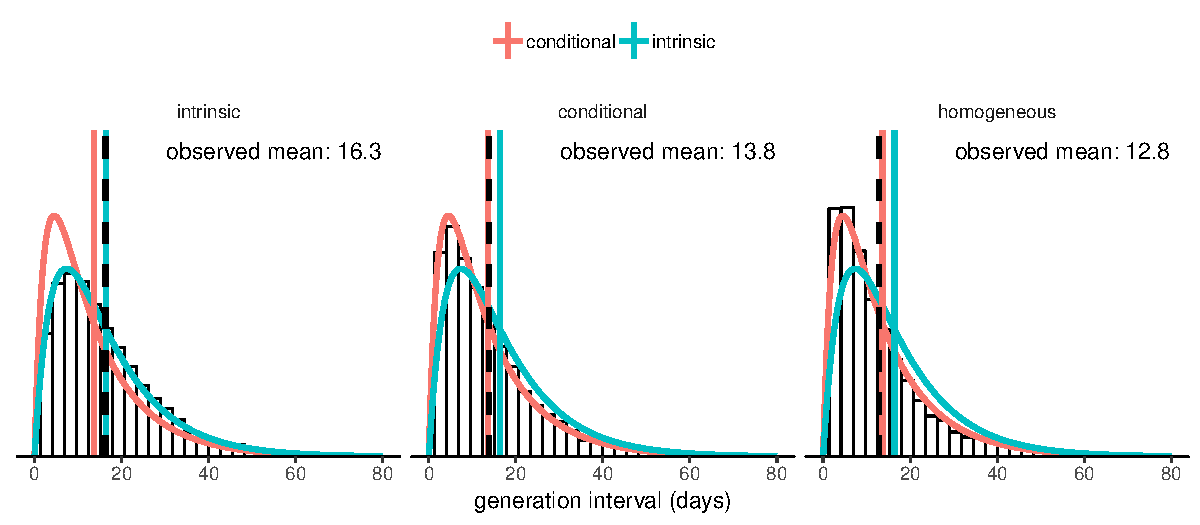
\includegraphics[width=\textwidth]{../fig/local_effect.pdf}
\caption{Fill this out.}
\label{fig:local}
\end{figure}

The egocentric generation interval \eqref{conditional} only explains some of the reduction in generation times that occurs on most networks, however.
Generation intervals are also shortened by indirect connections: a susceptible individual can be infected through another route before the focal individual makes infectious contacts.
Simulations on a small homogeneous network confirm this additional effect (\fref{local}, right panel). 
In general, estimating the effects of most networks on observed generation intervals is expected to be a hard problem. 

\subsection{Linking growth rate and reproductive number}



\section{Statistical approach to inferring generation-interval distribution}

It is clear that aggregating generation intervals through space and time yields a distribution that is different from the intrinsic distribution.
When the epidemic is growing, the proportion of susceptible individuals remain approximately constant and the intrinsic (or conditional) generation-interval distributions can be inferred from the observed intervals.
In this section, we investigate two statistical methods for recovering the intrinsic (or conditional) generation-interval distribution.
Detailed derivations of the two methods can be found in section.

\swp{maybe call it something else besides nonparametric method; it's still possible to make assumptions about the distribution and make inference}
We refer to the first method as the population-level method as it relies on the observed distribution without taking into account who infected whom.
As the observed generation-interval distribution is a weighted distribution of the intrinsic distribution, the intrinsic distribution can be recovered by taking the inverse of the weights, given by \eref{exp}.
Hence, the population-level method relies on the observed generation intervals and the exponential growth rate:
\begin{equation}
g(\tau) \propto \tsub{c}{exp}(\tau) \exp(r\tau).
\end{equation}

While the non-parametric method is simple, it does not use all available information from contact tracing data: it does not take into account who infected whom.
Assuming that infection occur as a poisson process in the beginning of an epidemic, we can obtain the following likelihood for the observed infection process:
\begin{equation}
\mathcal{L}(\RR, \theta) = \prod_{j=1}^N \left(\RR^{n_j} \exp \left(- \RR \int_0^{\tsub{t}{censor} - t_j} g(s;\theta) ds \right) \prod_{i=1}^{n_j} g(\tau_{i, j}; \theta) \right),
\end{equation}
where $N$ is the total number of infected individuals, $n_j$ is the number of individuals infected by $j$, $\tsub{t}{censor}$ is the time period which censoring was performed until, $t_j$ is the time at which infector $j$ was infected, $\tau_{i,j}$ is the observed generation interval between infector $j$ and infectee $i$, and $\theta$ is the (vector) parameter of the generation interval distribution $g$.
A similar method was proposed by \cite{forsberg2008likelihood} but it relies on discretized incidence reports rather than the observed generation intervals.

\swp{I might say something about independence transmission events in the results if I decide to compare forsberg2008 as well -- see forsberg 2008...}
\swp{I got stuck on forsberg 2008. I get weird estimates with wide confidence intervals but I feel like that's what their method is supposed to do (based on figure 3 in their paper). It doesn't use generation interval either so I think we can just ignore it?}

First, we compare how the estimates from the two methods vary across time using a single stochastic simulation on a homogeneous network (Figure~\ref{fig:example}).
During the initial exponential growth period (approximately between 9 and 20 weeks), both nonparametric and parametric methods yield similar estimates of mean generation interval and reproductive number.
However, we observe opposite trends after the growth period (approximately after 20 weeks).
As the nonparametric method takes a weighted average of the observed distribution, increase in the observed mean generation interval leads to increase in the nonparametric estimates of both mean generation interval and reproductive number.
On the other hand, as the parametric method assumes a Poisson process with constant proportion of susceptibles, decrease in the number of susceptible results in underestimation of both mean generation interval and reproductive number.
we observe grdaual increase in the observed mean-generation interval as we aggregate more data, but the observed estimates always underestimate both mean generation interval and reproductive number, as predicted from the deterministic simulation.

\begin{figure}
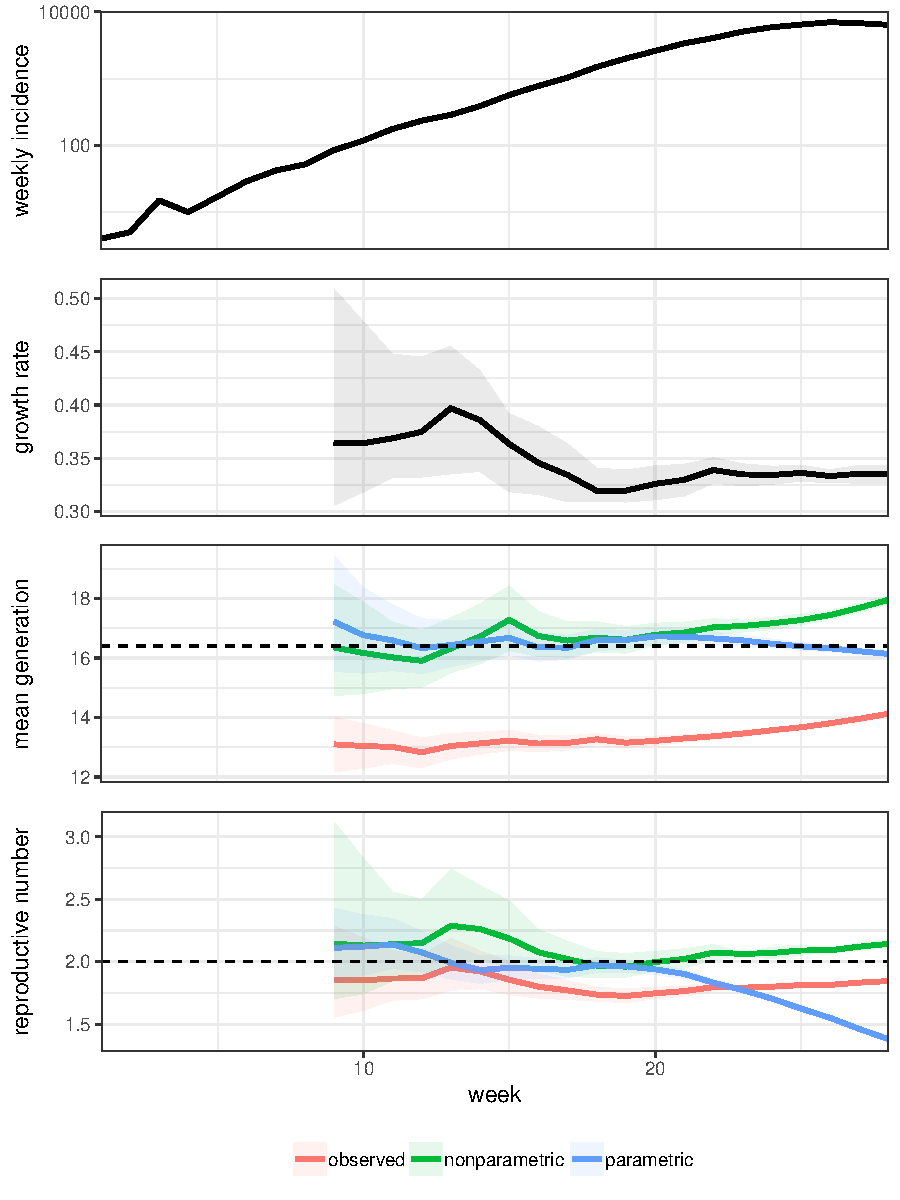
\includegraphics[width=\textwidth]{../fig/example.pdf}
\caption{Fill this out.}
\label{fig:example}
\end{figure}

Then, we compare accuracy and reliability of the two methods during the initial growth period using 100 stochastic simulations on a homogeneous network (Figure~\ref{fig:test}).
We find that the parametric method provides the most consistent (least variable) estimates.
The nonparametric method overestimates reproductive number initially but this is likely driven by the initial overestimation of the growth rate (Figure~\ref{fig:example}).


\swp{May need to explain what coverage is...}
Surprisingly, both methods fail to attain nominal coverage;
throughout the estimation period, both methods attain approximately 70\% coverage.
Even though the gamma distribution looks indistinguishable from the shape of the intrinsic generation-interval distribution, making a wrong distributional assumption leads to underconfidence.
To confirm that the undercoverage is caused by distribuional assumption, we simulated an epidemic using gamma kernel and found that using the true shape yields nominal coverage (see Appendix).
These results are particularly alarming because shape of the generation-interval distribution have often been assumed in outbreak analyses and it is impossible to know the true shape of the distribution [CITE].
\swp{Why does nonparametric method undercover?}

\begin{figure}
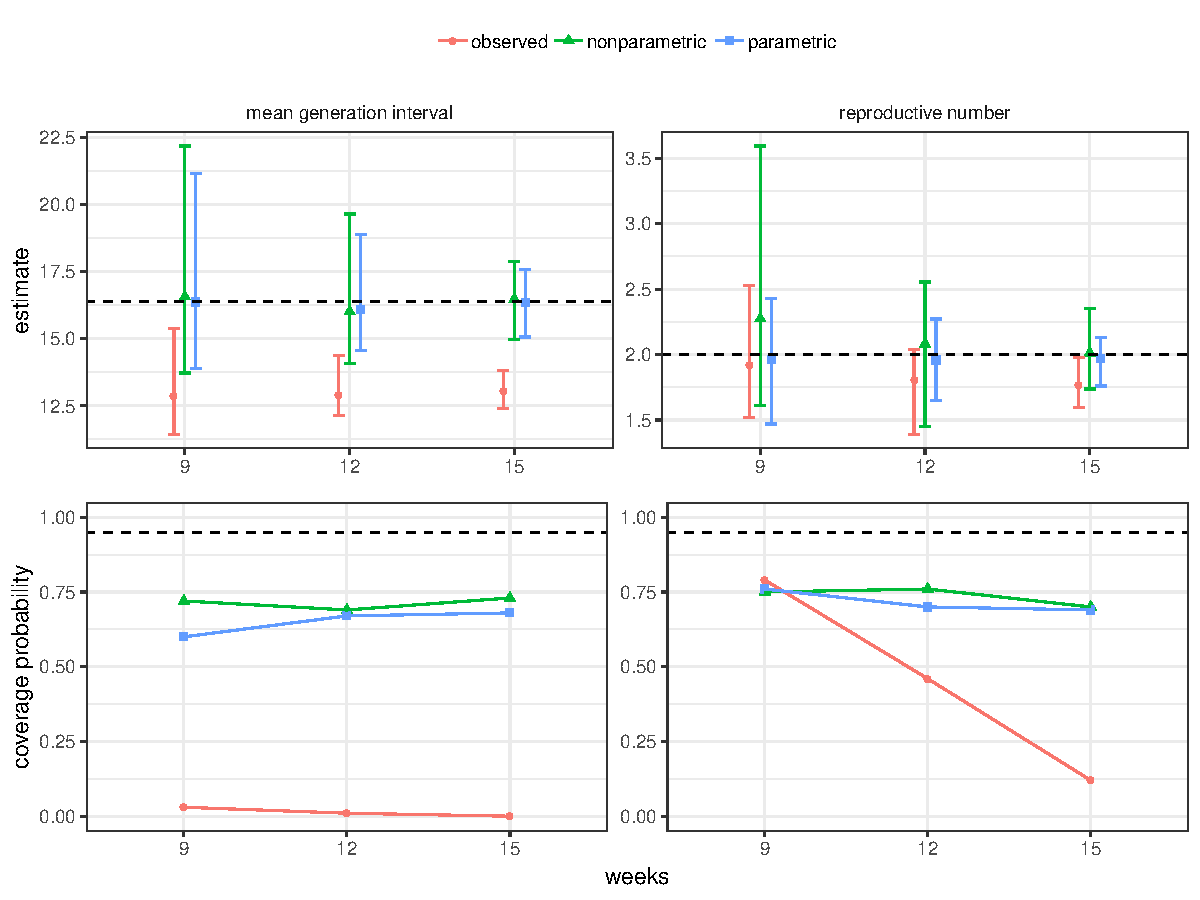
\includegraphics[width=\textwidth]{../fig/compare_methods.pdf}
\caption{Fill this out.}
\label{fig:test}
\end{figure}

\clearpage

\section{Discussion}

\section{Methods}

The first method is a non-parametric method.
Recall that the observed generation-interval distribution is a weighted intrinsic generation-interval distribution (equation~\ref{eq:obsg}). 
Then, the intrinsic generation-interval distribution can be obtained by taking the inverse weight:
\begin{equation}
g(\tau) \propto c_t(\tau) \frac{1}{\int_{0}^t i(s-\tau) S(s) ds}
\end{equation}
However, this method requires a knowledge of susceptible dynamics and may difficult to use in practice.
Instead, during the exponential period, the generation-interval distribution is
\begin{equation}
g(\tau) \propto \tsub{c}{exp}(\tau) \exp(r\tau)
\end{equation}
and the reproductive number is
\begin{equation}
\RR = \int \tsub{c}{exp}(\tau) \exp(r\tau) d\tau.
\end{equation}
Note that applying the Lotka-Euler equation directly to the observed generation intervals will always underestimate the reproductive number:
\begin{equation}
\int_0^\infty \tsub{g}{exp}(\tau) \exp(r\tau) d\tau > \left(\int_0^\infty \tsub{g}{exp}(\tau). \exp(-r\tau) d\tau\right)^{-1}
\end{equation}

Finally, we obtain an estimator for mean generation interval and the reproductive number:
\begin{equation}
\begin{aligned}
\hat{G} &= \frac{\sum_{i} \exp(r c_i) c_i}{\sum_{i} \exp(r c_i)},\\
\hat{\RR} &= \sum_{i} \exp(r c_i),
\end{aligned}
\end{equation}
where $r$ is the exponential growth rate and $c_i$ is an individual generation interval sample.

\bibliography{network}
\end{document}
